%%%%%%%%%%%%%%%%%%%%%%%
%%      Lecon 2      %%
%%%%%%%%%%%%%%%%%%%%%%%

\chapter{Des subprimes à Fortis : La contamination du système financier mondial}
\section{Marché immobilier aux USA}
\begin{wrapfigure}[9]{l}{8cm}
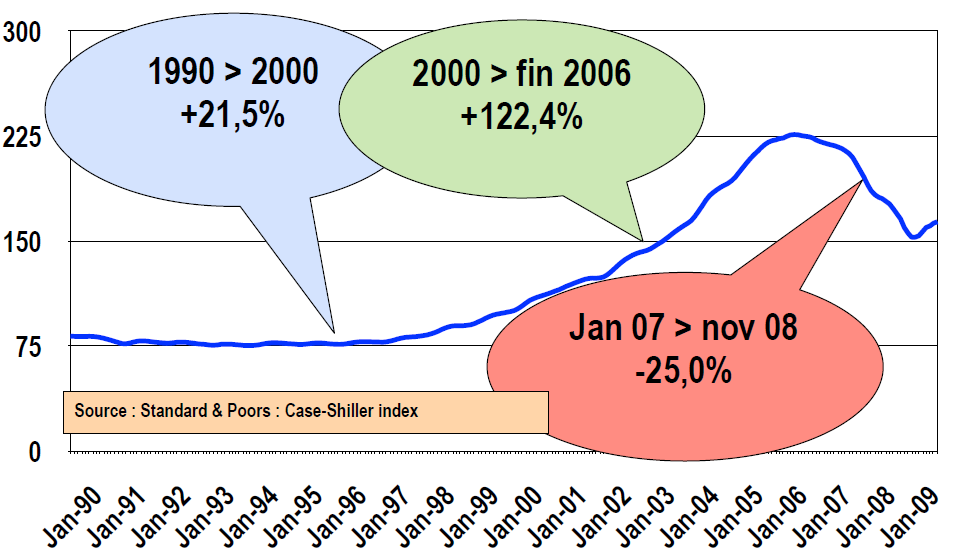
\includegraphics[scale=0.3]{2}
\end{wrapfigure}
\ \\ Comme on peut le voir selon \textbf{l'indice Case-Shiller} \footnote{Outil de mesure de la valeur de l'immobilier important.}, pendant 10 ans la valeur de l'immobilier reste stable. S'en suit une période de 4 ans où la valeur de l'immobilier explose pour finir en chute libre. Les deux premières étapes s'étendent sur une longue durée mais la chute se manifeste par la perte de 25\% de valeur en $\pm$ 1 an !

\begin{wrapfigure}[10]{l}{8cm}
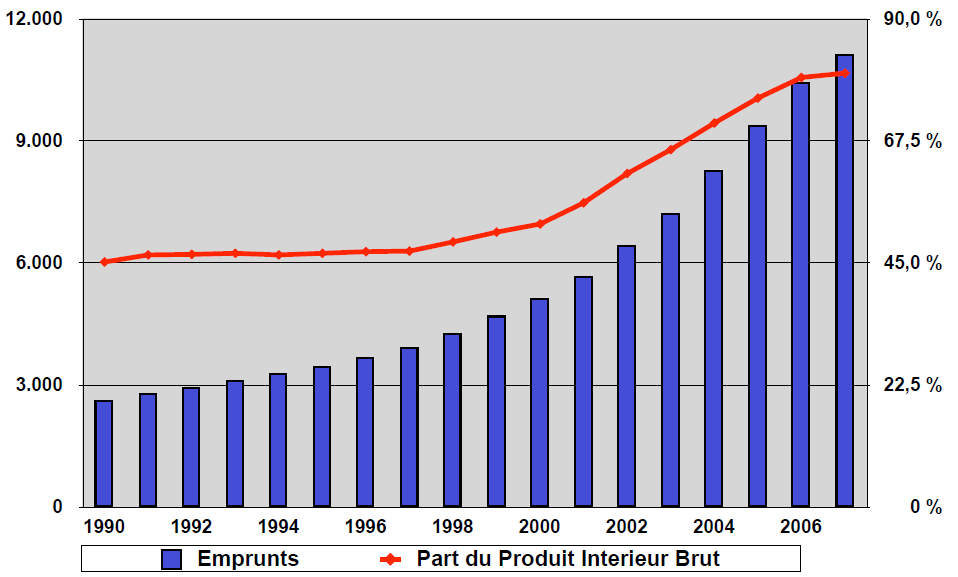
\includegraphics[scale=0.3]{3}
\end{wrapfigure}
\ \\ Si on analyse l'évolution des emprunts durant cette période, on peut constater qu'on a réussi à refiler de plus en plus de crédit. Ceci ravi les banquiers qui ont beaucoup d'argent à distribuer. On observe aussi une explosion de l'emprunt aux alentours de 2002 mais en contre partie, on peut voir que les emprunts ont atteint les 90\% du PIB et donc que celles-ci pèsent sur les ménages. 

\section{L'effet de levier}
On avait vu au premier chapitre que l'objectif de tout investisseur était de maximiser la rentabilité de son investissement. Pour ça, il va donc faire attention non seulement aux \textbf{revenus} (loyer, intérêt, ...) mais il va aussi faire attention à ce que la valeur de revente soit plus élevée \textbf{(plus-value)}. Cependant, selon la loi de la finance (c'est démontrable), une rentabilité élevée signifie un risque élevé. Et donc l'investisseur va essayer de maximiser la rentabilité et minimiser le risque. Pour ça, il a le principe de \textbf{effet levier} :

\begin{wrapfigure}[10]{l}{9cm}
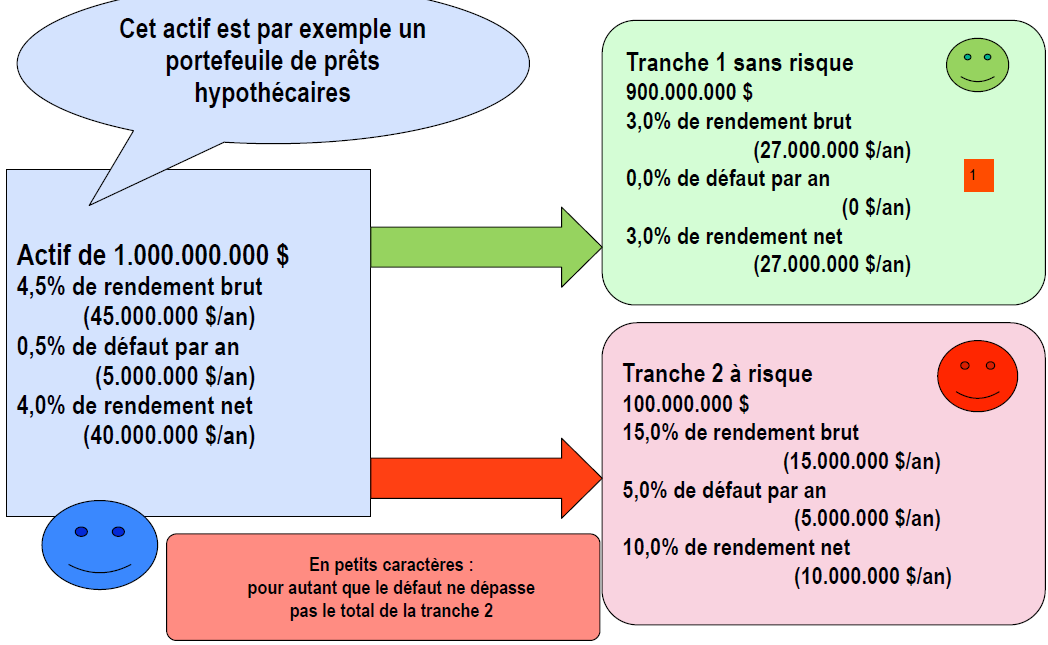
\includegraphics[scale=0.3]{4}
\end{wrapfigure}
Le principe est simple, considérons un investisseurs disposant d'une grande somme d'argent. Il va investir la totalité et aura un revenu brut mais aussi un certain défaut parce qu'il est possible que quelqu'un ne puisse pas rembourser à temps. Pour minimiser le risque et maximiser le gain, il divise le capital en 2 tranches :
\\
\begin{enumerate}
\item Une première tranche qui consiste en 90\% du capital et qui sera investit sans risque (on considère que c'est garantit) mais avec un gain faible.

\item Une deuxième tranche qui constitue le reste du capital qui est investit à haut risque et donc qui rapportera gros. 
\end{enumerate}
Donc tout le monde est gagnant et tout le monde est content. 

\section{Innovation financière}
Pour appliquer à fond l'effet de levier, on invente les \textbf{CMO} (Collateralized Mortgage Obligations - 1983) \footnote{Emprunts couverts par des prêts hypothécaires mis en gage.} et \textbf{CDO} (Collateralized Debt Obligations - 1987) \footnote{Emprunts couverts par tout type de dette mises en gage.}. De plus, on découpe le porte feuille en de très nombreuses tranches de risque (comme en haut). Ceci change complètement le métier du crédit parce qu'avant, une seule institution se chargeait de toutes les fonctions (suivi du crédit, ...), la banque intégrée. Mais avec ces pratiques, différentes institutions gèrent différentes fonctions. Ceux-ci sont repris dans le tableau ci-dessous avec leurs conséquences à côté.

\begin{center}
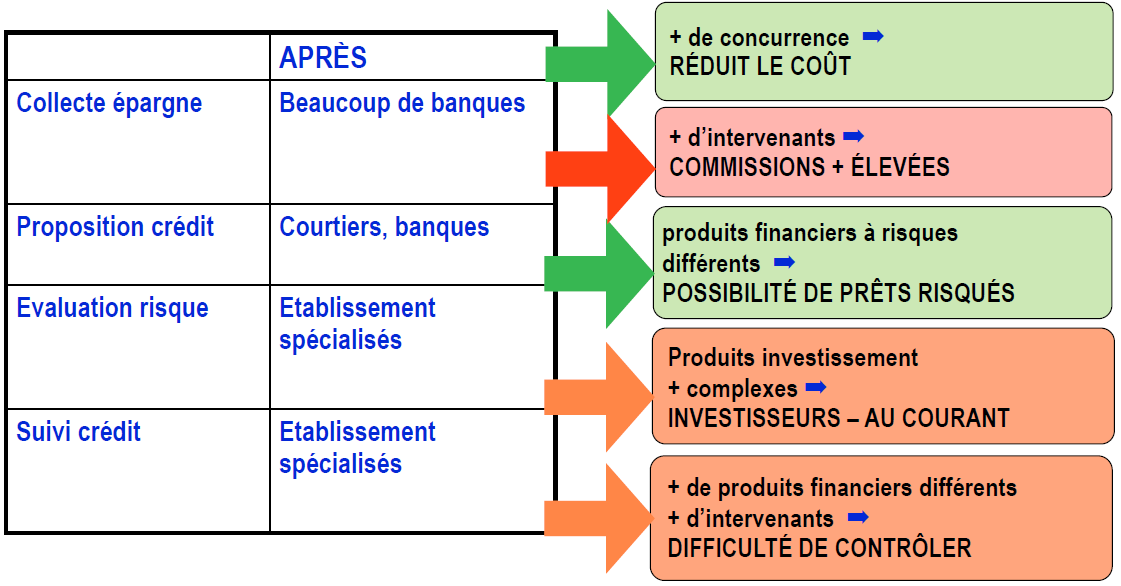
\includegraphics[scale=0.4]{5}
\end{center}

On voit donc qu'en fait on commence à perdre le contrôle sur la finance en raison de cette division. 

\section{Le boom immobilier américain}
Comme on le sait déjà, il y a eu, vers les années 50', une migration massive de la campagnes vers les villes (en Europe et USA). En Asie, elle est venu plus tard, vers les années 90'. Après ce mouvement, il y a eu une certaine migration vers les banlieues\footnote{"Nostalgie des banlieues"} vers les années 70'. Ajoutons à cela, l'explosion démographique entre 1940-45 en Europe et aux USA. \footnote{En gros tous les batards de la guerre ... "Baby boom"}. Mais aux USA, on a encore un phénomène qui stimule l'immobilier qui est la finance. En effet, comme on l'a vu, il y a une offre abondante des banques avec des taux d'intérêts faible. Puisque les ménages n'ont pas vu leur salaire augmenté, on a anticipé la croissance à l'aide d'un principe appelé \textbf{Irrational exubérence} qui est un principe très optimiste sur l'avenir. Cette notion est illustrée sur la figure ci-dessous.

\begin{center}
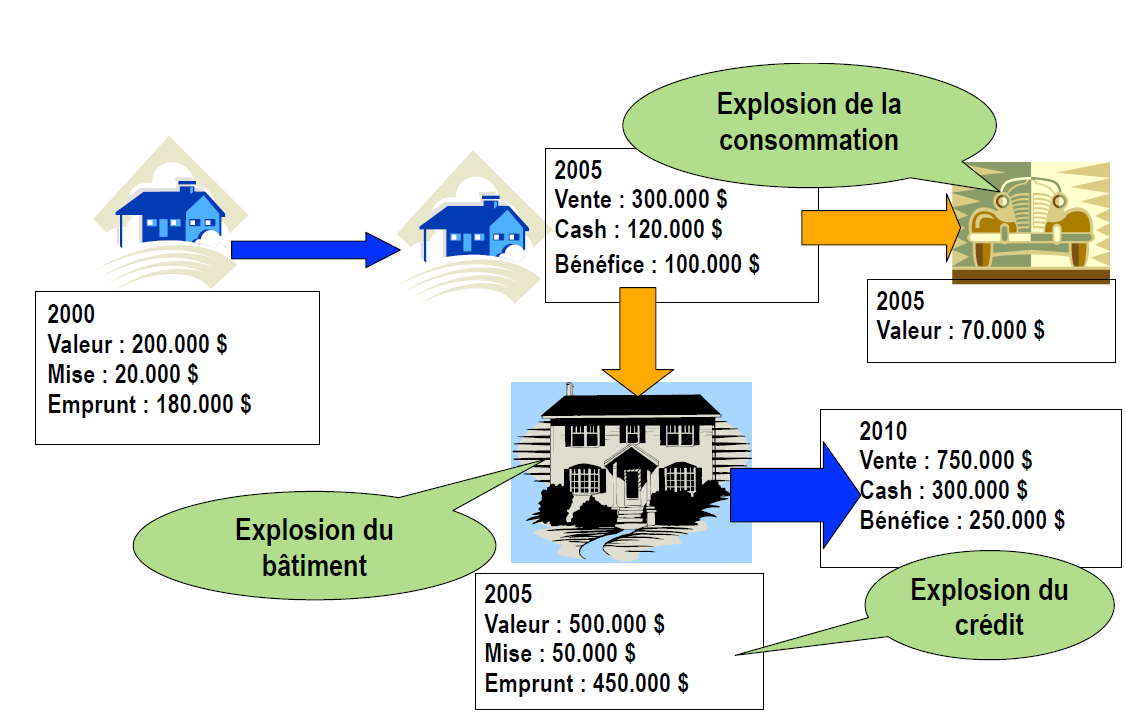
\includegraphics[scale=0.4]{6}
\end{center} 

C'est optimiste car on suppose que la valeur de l'immobilier ne fera qu'augmenter et donc on commence avec petit, ça prend de la valeur, on vend, on a gagné de l'argent donc on peut viser plus grand (plus grand crédit) et dépenser son argent dans d'autre produits et la roue tourne.

\section{Nouvelles innovations financières}
Cependant, si la demande ne suit pas, c'est à dire si les gens n'empruntent pas, ça ne va pas ! C'est pour ça qu'est apparu différentes facilités : taux variable, pas de remboursement du capital ou des intérêts\footnote{"Interest only mortgage"}, options de payement flexible \footnote{Principale remboursé si possible.}, on ne fait plus très attention à la valeur du bien, aux revenus ou au budget du ménage (sub-prime), on peut même aller jusqu'à ne plus faire d'enquête (Alt-A) et on instaure les prêts de longues durées (40 ans et plus) ainsi que les \textbf{emprunts inversé} \footnote{Lorsqu'on décède, on cède le bien à la banque.}. 
\\\\
Tout ceci a pour conséquence que l'immobilier progrèsse très bien (de 122 \% de 2000 à 2006) mais l'innovation financière fait en sorte que les sub-primes et Alt-A prennent une place de plus en plus importante dans le crédit (laisser-aller progressif). 
\\\\
Pour finir, l'effet de levier peut évoluer en \textbf{Hedge Funds} qui ne sont rien d'autres que des fonds à effet de levier maximum. "Hedging" signifie en finance un instrument de sauvegarde ou de protection contre les limites de risque. Il s'agit, par exemple, d'un produit financier qui protège contre les augmentations de taux d'intérêt au-delà de certaines limites. Le principe consiste, par exemple, à investir 100 euro mais on emprunte 400 euro à la banque pour investir 500 euro. De cette manière, on utilise là une première fois l'effet levier. On peut aussi iinvestir dans les CDO qui eux aussi utilise l'effet levier ! On a donc un double effet levier. Les bénnéfices sont donc beaucoup plus élevés mais au détriment du risque qui prend une plus grande importance également. 
\\\\
On a donc là fait le bilan de toutes les innovations : 
 Les instruments de "Hedging" offrent souvent, pour la même mise de fonds, des perspectives de rendement plus élevées. avec, à la clé, plus de risques (ce dont les investisseurs ne sont pas toujours conscients).
Les "Hedge Funds" investissent en principe majoritairement dans ce type de produit.
Quand je dis utiliser soi-même l'effet de levier, j'entends que généralement les "Hedge Funds" s'endettent. En outre ils investissement fréquemment dans des produits de type CDO qui utilisent à leur tour l'effet de levier ! Il y a donc double effet de levier
\begin{enumerate}
\item \textbf{Sub-prime} : on a prêté massivement sans se soucier du remboursement.

\item \textbf{Effet de levier} : on donne du haut rendement aux emprunts risqués et on vend, comme sans risque, la grande masse des emprunts. 

\item \textbf{CDO} : les produits mis en gages sont de pllus en plus sophistiqué et transparents (j'imagine que ça veut dire que c'est plus difficile à vendre).

\item \textbf{Hedge Fund} : les investisseurs se sont endettés à leur tour pour acheter des CDO et donc faire leur propre effet de levier.
\end{enumerate}

\section{Déclin}
\subsection{Ralph Cioffi}
Si on revient en juin 2007, ça craque pour deux fonds qu'il gère. Les fonds, investits en CDO appartiennent à la banque \textbf{Bear Stearns}. Ils empruntent donc chez Merril Lynch. Puis ça s'effondre ! La valeur des CDO diminue et Merril Lynch procède à un appel de marge de 145 millions de dollars. Bear Stearns n'arrive pas à vendre les CDO et Merril les réquisitionne. Sauf que lui non plus n'arrive pas à les vendre. Bear Stearns licencie Cioffi et réinjecte 3,2 miliards de dollars. \\
En août et septembre, plusieurs grandes banques annoncent des pertes sur les sub-primes (20 milliards). \\
En novembre, ces estimations de pertes ont explosé ! On est passé de 20 milliards à 400 ou 500 milliards de dollars ! \\
Un analyste a demandé à Garry Grittenden si la vague de dépréciations étaient finies. La réponse a été très incertaine. Ceci montre que la situation n'est plus sous contrôle. 

\subsection{Piliers de la banque}
Le pilier d'une banque c'est bien sûr la confiance. Cette confiance doit être attribué par : 
\begin{enumerate}
\item \textbf{Les épargnants} : c'est des clients que vient l'argent, donc source primaire de financement.
\item \textbf{Les autres banquiers} : il y a des échanges interbancaires quotidiens.
\item \textbf{Les actionnaires} : qui investissent dans la banque et qui sont souvent épargnants.
\item \textbf{Le personnel} : qui sont souvent aussi actionnaires et épargnants. 
\end{enumerate}

\subsection{La banqueroute de Stearns}
Après Cioffi, ils annoncent plusieurs fois des pertes et l'action en bourse s'est effondrée (passse de 170 à 10 dollars l'unité !). Suite à cela, les épargnant retirent leur dépôts et les autres banques refusent de prêter de l'argent. Finalement, on fait appel à la US Federal Reserve \footnote{US Federal Reserve : Banque Central américaine. Orgaanisme chargé d'émettre la monnaie, de contrôler les banques et de veiller au bon fonctionnement du système bancaire. Il soutient, moyennant conditions, les banques en difficultées.} (plus assez de liquidité) qui organise la reprise de Bear Stearns.

\section{Pouvait-on prévoir ?}
\subsection{Charles Morris}
Il écrit un livre en automne 2007 et le publie au printemps 2008. Il y annonce \textbf{"la mère de tous les krachs"} pour la mi-2008. Son raisonnement se base sur l'effondrement progressif de la confiance qui est causé par la crise des sub-primes. Il démonte les mécanisme d'organisation du système bancaire ayant conduis à l'innovation sans limite, les crédits hypothécaires sans limites et le développement des produits non contrôlés.

\subsection{Nouriel Roubeini}
C'est un professeur de la Stern School à New York. Déjà en septembre 2006, Roubeini annonçait au FMI \footnote{Fonds Monétaire International} q'une grande crise arrivait aux USA. Mais déjà avant, il avait prévu l'explosion de la bulle technologique en 2000. Ses 12 étapes de la crise sont repris ci-dessous.  
\begin{center}
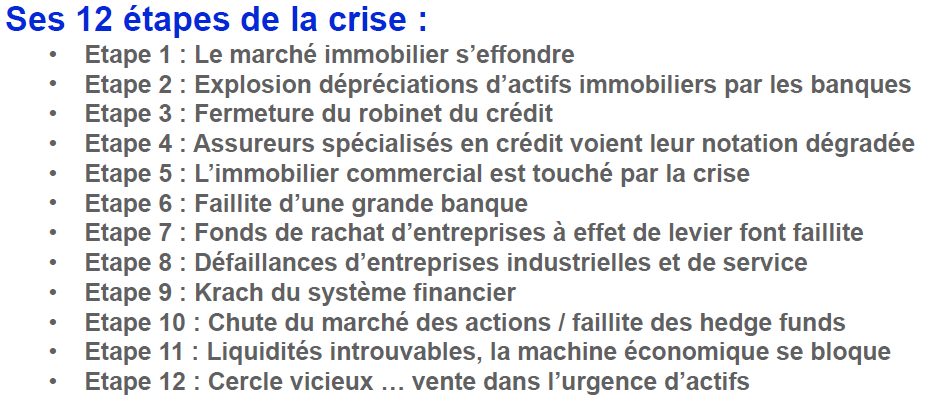
\includegraphics[scale=0.4]{7}
\end{center}

\subsection{Mais beaucoup rassuraient}
Même les organismes publics de contrôlent ne se doutaientt pas que la crise était possible. Une étude du FDIC \footnote{Federal Deposit Insurance Corporation : Institution publique américaine chargée d'assurer les consommateurs en cas de faillite d'une institution bancaire ou financière.} à l'été 2006 constate qu'il y a un développement rapide des produits non traditionnels ainsi que leur extension à des clients à profil risqué (les ménages à bas revenus) mais le plus important, l'augmentation de la valeur de l'immobilier qui limite les risques en cas de défaut. \\
On voit qu'en fait on a accumuler d'énormes risques en pensant que c'était sans risque.

\section{Faillite des grandes banques}
On a cru pendant longtemps qu'il était impossible qu'une grande banque fasse faillite parce que ça destabiliserai le système économique du pays. Aux USA, des petites et moyennes banques ont fait faillite mais on été reprises par d'autres banques et les épargnants n'ont rien perdu grâce à l'intervention de l'Etat (ce sont les actionnaires qui perdaient). En Europe, c'est moins fréquent et on a une meilleure protection des épargnants. Par contre, dans des pays moins développés, c'est très fréquent et les ce n'est pas toujours sans conséquence pour les épargnants. 

\subsubsection{Faillite de Lehman Brothers}
C'était une des 10 plus grandes banques américaines. Mais ils ont réalisé des pertes considérables sur à cause des sub-primes (20 milliards de dollars) et comme précédemment, les épargnants retirent leur argent et les autres banques refusent de prêter. \\
Une réunions des grandes banques américaines a été organisé sous la tutelle des autorités fédérales mais aucune banque ne veut reprendre Lehman sans une aide fédérale massive. Les autorités américaines refusent car l'aide est trop importante. Ce qui a conduit à la faillite de la banque. 

\section{La belle histoire de Fortis}
Une étape importante dans leur histoire a été l'acquisition d'ABN-AMRO. Celle-ci était un groupe financier hollandais diversié (banque et assurance) dont l'action en bourse évolue moins bien que les autres banques européennes. Les actionnaires sont donc mécontents (pas assez rentable) et mettent le management sous pression pour qu'ils vendent l'entreprise (on peut gagner beaucoup d'argent). La première offre de 61 milliards \$ vient de la banque anglaise Barclays. \\
C'est la que Merill Lynch propose une idée. C'était de diviser l'entreprise entre 3 investisseurs et chacun prendrait la part qui l'intéresse afin de rentabiliser les parts le plus rapidement possible. A l'époque tout le monde y croyait et on se doutait pas du risque des sub-primes. (exhubérance irrationnelle). Il suffisait donc de proposé plus que Barclays. 71 milliards \$ a été proposé par les 3 banques : Royal Banque of Scotland, Fortis et Santander. En Août 2007, les conquérants l'emportent. 

\section{Fortis et la finance mondiale}
Afin de comprendre la raison de cet achat par Fortis, regardons un peu l'histoire de cette banque qui est reprise sur les deux figures ci-dessous.\\
\begin{minipage}{0.55\textwidth}
\begin{flushleft}
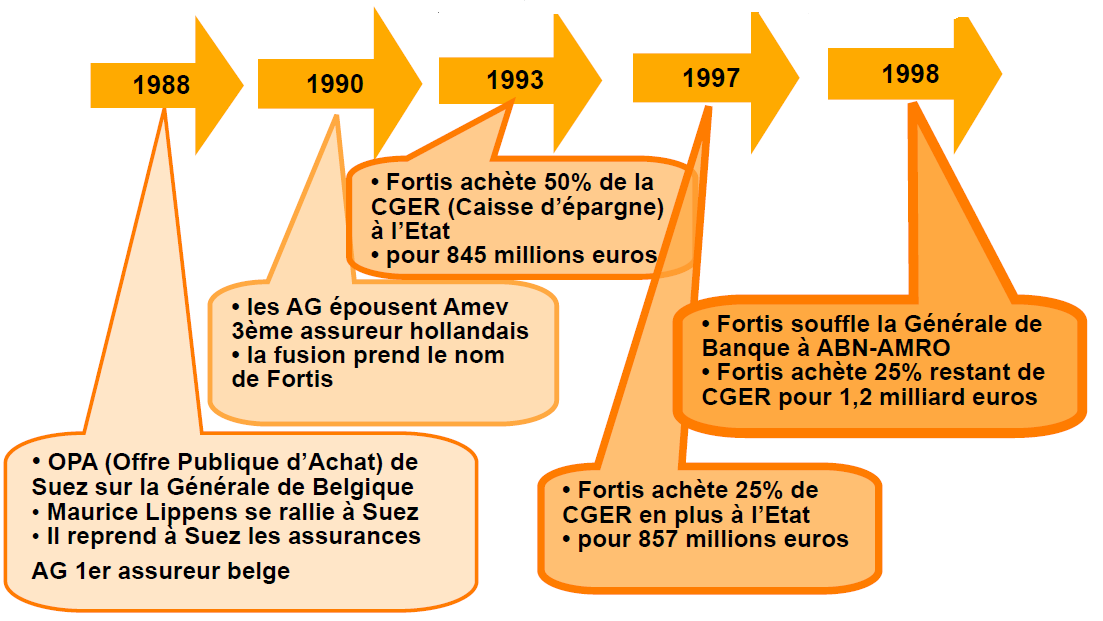
\includegraphics[scale=0.3]{8}
\end{flushleft}
\end{minipage} 
\begin{minipage}{0.5\textwidth}
\begin{flushright}

\includegraphics[scale=0.3]{9}
\end{flushright}
\end{minipage} \\

Leurs motivations son repris en ces points : 
\begin{itemize}
\item \textbf{Sortir des frontières} : il ne faut pas rester qu'en Belgique. Il faut s'étendre pour avoir de plus grand marchés $\rightarrow$ mondialisation.

\item \textbf{Acheter plutôt qu'être racheté} : si on est petit on se fera racheter par les plus grands. Donc il y a une certaine course à la taille. De plus, une même opération coûtent moins cher lorsqu'elle est reproduite en masse (comme dans l'industrie). Tout est informatisé donc le coût du système informatique reste inchangé quel que soit le nombre de clients également. Les produits est le même que ce soit en Belgique ou un autre pays. 

\item \textbf{La Banc-assurance} : l'assurance et la banque étant deux activités financières très proches, il y a un souhait de regroupement. Ceci permettrait non seulement de vendre ces deux produits aux mêmes guichets mais également d'utiliser les placements des assurances pour développer la banque.

\item \textbf{Grandir :} désir de passer d'une banque locale intégrée en une  banque international de marché. 

\item \textbf{Conservation du marché} : on veut attirer le plus de clients possible en transformant les entreprises poussiéreuse en quelque chose de rentable au maximum pour l'actionnaire.
\end{itemize}

Historiquement, Fortis désire passer d'une société privée conservatrice à une institution publique de crédit (à vérifier). Cependant, l'actionnaire classique considère toujours Fortis comme l'ancienne Générale de Belgique où les actionnaires sont des "bons pères de famille". Alors que les actionnaires internationnaux ont des exigences fote en matière de rentabilité et de prise de risque élevé. Donc, ça le motive également à aller chercher ailleurs. \\
Fortis devient l'une des 20 plus grandes banques mondiales et l'une des 10 plus granddes en Europe. \\
La banque grandit jusqu'à gérer des acifs d'une valeur de 410 milliards d'euros en 2007 et la valeur des produits générés a atteint 25 milliards d'euros (slide 9). 

\begin{wrapfigure}[8]{l}{8.5 cm}
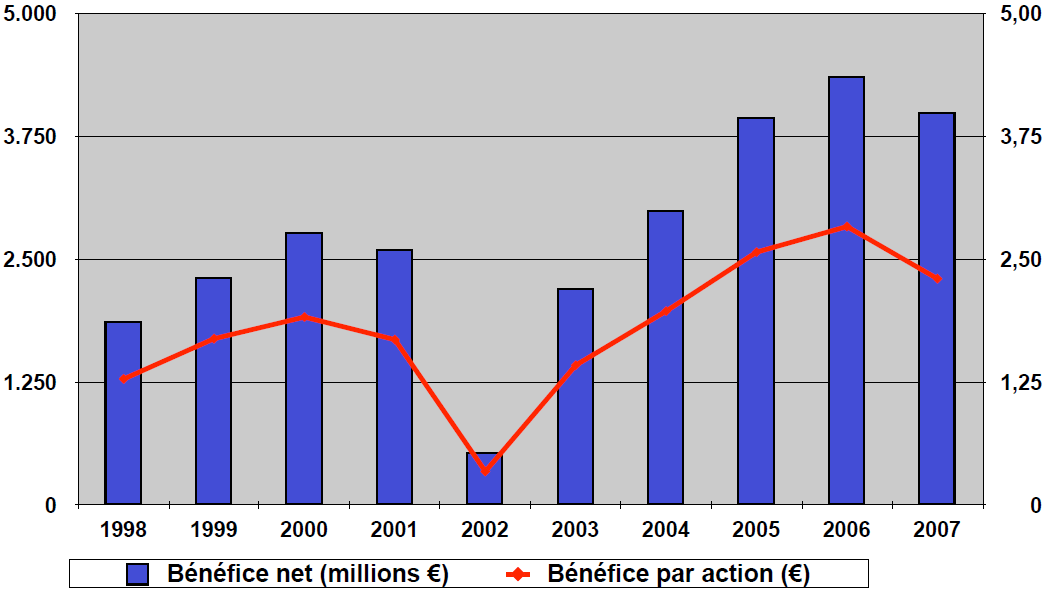
\includegraphics[scale=0.3]{10}
\end{wrapfigure}
\ \\ Cepedant, si on regarde le graphe ci-contre, on remarque qu'il existe une défaillance en 2002. Le bénéfice net et le bénéfice par action ont dégringolé malgré une évolution constante de la taille de la banque. Cette acciddent en 2002 a eu des conséquences diretes sur la valeur de l'action. 

\begin{wrapfigure}[10]{l}{8.5 cm}
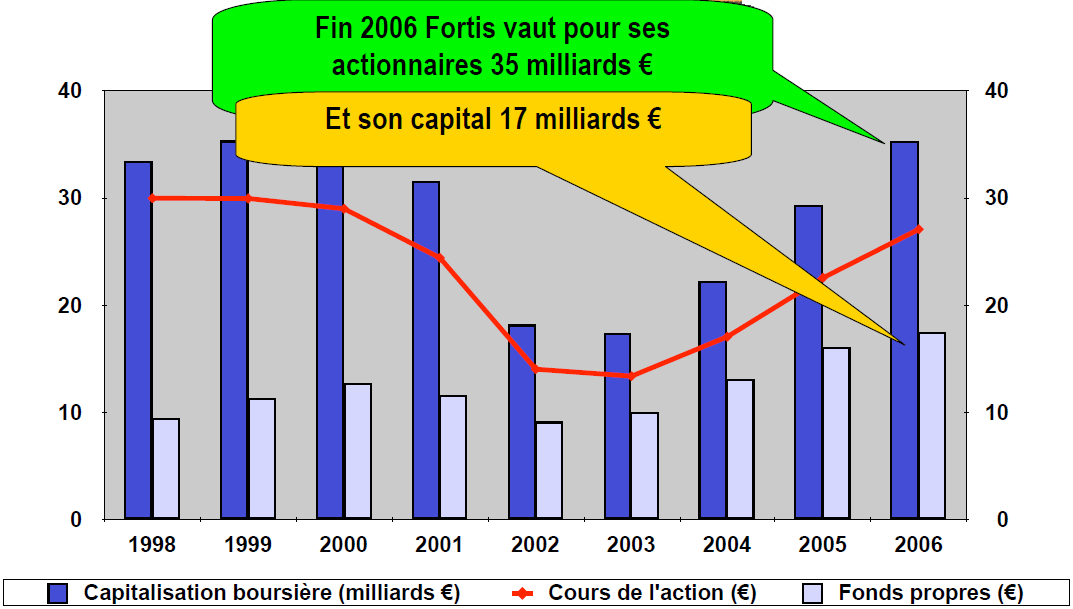
\includegraphics[scale=0.3]{11}
\end{wrapfigure}
\ \\ Quand on acquiert des actions, on espère qu'après un certain temps leur valeur augmentera. Cependant, pour Fortis, malgré la très bonne évolution, le cours de l'action est retombé entre 1998 et 2006. Fortis ne vaut en 2006, pour ces actionnaires, que ce qu'elle valait aproximativement en 1998 (35 milliards). Bien sûr, les actionnaires ne sont pas content. 

\section{ABN-AMRO, facteurs peu logiques}
Revenons à cette acquisition et montrons les facteurs pas très logiques. 
\begin{itemize}
\item Si on refait l'état des lieux, Fortis vaut 35 milliards en bourse, son capital s'élève à 17 milliards et l'acquisition est de 24 milliards d'euros. C'est donc fou de se lancer dans une telle affaire! Mais elle est devenu n\degres 1 au Benelux : première banque, première assurance avec un Benelux qui compte 28 millions d'habitants dont le revenu fait partie des plus élevé. Elle est aussi l'une des 10 premières banques au monde pour les actifs en gestion \footnote{Les sommes confiées à la banque} mais aussi pour la gestion de fortune. 

\item Fortis expliquait vouloir s'étendre hors du Benelux. Or, là c'est tout le contraire qui se passe.

\item La commision européenne va exiger des cessions (vendre une partie de ce qu'on acquiert) pour éviter que Fortis ne soit trop dominant sur le marché du Benelux. De plus, il y a un risque à la revente parce que les délais de payement sont courts (pour l'acquisition).

\item Intégrer une grande banque sera difficile en raison des rivalité Fortis >< ABN-AMRO, des rivalités culturelles et les risques opérationnels importants (intégration technique). La rivalité entre les deux banques a commencé lorsque ABN-AMRO voulait acquérir la Générale de banque mais que Fortis l'a emporté. Mais aussi parce que le CEO de Fortis \footnote{Jean-Paul Votron} a été le n\degres 2 de ABN-AMRO dans le temps et a toujours voulu devenir n\degres 1.
\end{itemize}
On peut donc penser qu'il y a certains facteur émotionnels dans l'acquisition. 

\section{Acquisition d'ABN-AMRO}
Il faut décaisser au total 24 milliards d'euros. Les actionnaires de Fortis doivent fournir 13.5 milliards (confiance des actionnaires), 5 milliards seront empruntés aux marchés (confiance des autres banques) et on va devoir revendre 5.5 milliards à cause de la cession de la commission européenne. Il va donc faloir trouver des acquéreurs au bon prix. De plus, il faut que tout se passe bien. Donc il ne faut pas d'accident au sein de l'entreprise, ni dans les marchés. \\

Les prises de décisions se passent comme suit : 
\begin{enumerate}
\item \textbf{Etude du projet} (début 2007) : par l'équipe de management et quelques administrateurs-clé. 

\item \textbf{Décision formelle d'y aller} (avril 2007) : par le conseil d'administration. 

\item \textbf{Décision de financement}(août 2007) : par l'Assemblée Générale Extraordinaire des actionnnaires.

\item \textbf{Assemblée Générale} (avril 2008) : C'est la que commence la dégringolade! "Décharge" (confiance) à tous les administrateurs et renouvellement de ceux-ci, dont Lippens et Votron (CEO).  

\item \textbf{Augmentation de capital d'urgence} (26 juin 2008) : décidé par 3 administrateurs sur un total de 13!!
\end{enumerate}

Afin de mieux comprendre la décision d'acquisition au sein de l'entreprise, un résumé du cadre professionelle dans une banque est disponible à la page suivante. 

\begin{center}
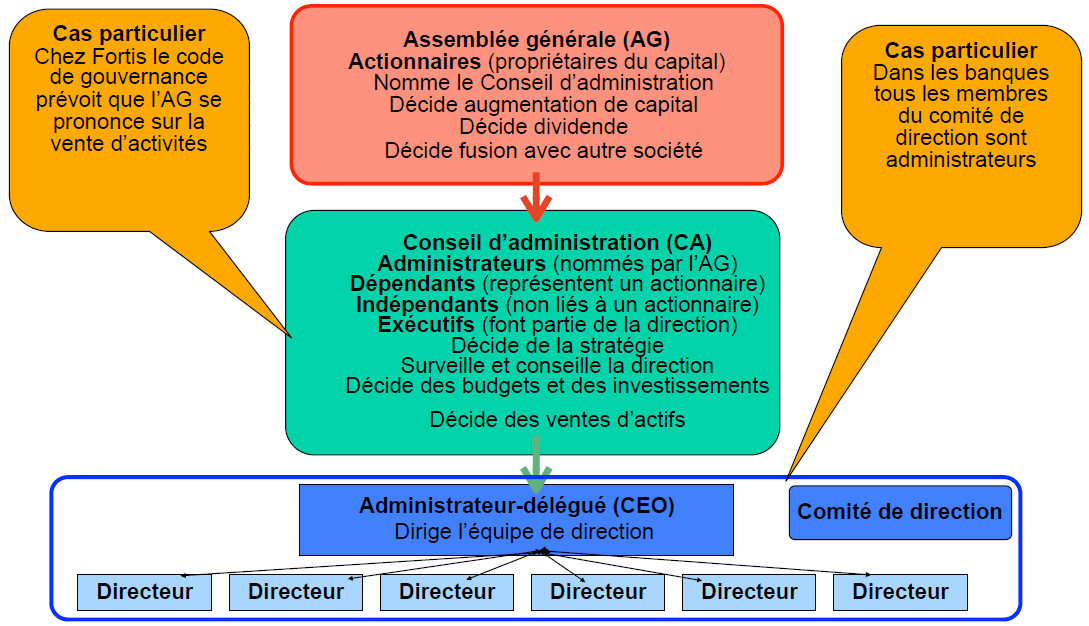
\includegraphics[scale=0.4]{12}
\end{center}

Voici maintenant un résumé de tous les événements qui se sont déroulé durant la chute de la valeur de l'action de Fortis. Comme on peut le constater, la chute va de pair avec la crise aux Etats-Unis. 

\begin{center}
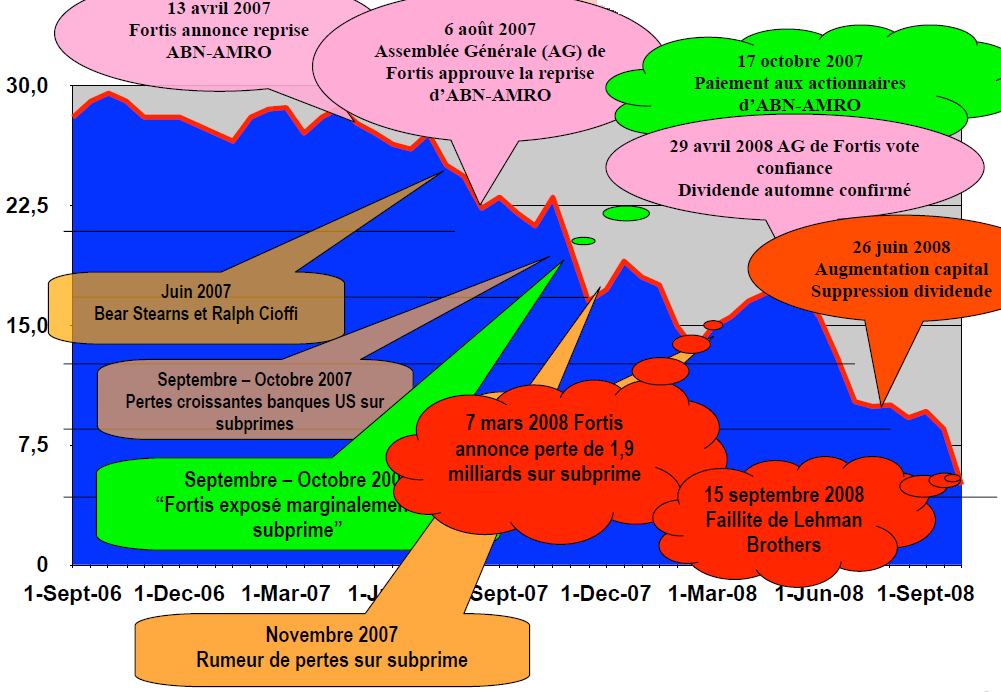
\includegraphics[scale=0.45]{13}
\end{center}

Durant cette fameuse chute, on a également une perte progressive de la confiance accordée à la banque. Les différentes raisons sont : 

\begin{itemize}
\item \textbf{Augmentations successives de capital :} Même phénomène que pour Lehman Brothers, la valeur de l'action perd de sa valeur (-33\% en 9 mois!). Ceci mène à une perte de confiance des actionnaires.

\item \textbf{Information tardive sur les subprimes :} On joue avec les actionnaires car on leur annonce 4 mois plus tard qu'il y a une perte conséquente à cause des subprimes! On peut voir sur le graphe du dessus que les pertes surviennent vers septembre - novembre 2007 mais que l'annonce passe le 7 mars 2008. 

\item \textbf{Instabilité des dirigeants :} Départ du directeur financier et du CEO alors qu'ils venaient d'être nommés pour 4 ans. 
\end{itemize}

A partir de septembre 2008, les particuliers commencent à retirer leur dépôt mais le plus important, c'est que les grandes entreprises également les retirent. On a une perte considérable de cash. Après ça, les difficultés dans l'interbancaires croissent. "Le prédateur est devenu proie". \\
Fortis est particulièrement touché par la faillite de Lehman Brothers parce qu'elle avait vendu massivement des produits de cette banque. A partir du 25 septembre, les liquidité ne suffisent plus \footnote{Les besoins sont estimés à 40 milliards d'euro pour le 29 septembre.} et donc c'est la fin de la route, les Etats doivent intervenir. \\
La Belgique, les Pays-Bas et le Luxembourg augmentent le capital des banques Fortis (Bel,NL,Lux) et deviennent propriétaires à 50\% de ces banques. \\
Même cela ne suffit pas! On lègue totalement Fortis NL et ABN-AMRO à l'Etat hollandais, on vend les 50\% restants de Fortis Belgium à l'Etat Belge et l'Etat revend 75\% de cette dernière à BNP Paribas.